\begin{frame}{Neue Wechselwirkung}
\begin{itemize}
	\setlength\itemsep{1em}
	\item Neue $U(1)$-Symmetrie mit Eichboson $Z'$ \cite{InColour}
	\item Unter der neuen Wechselwirkung geladene Teilchen:
	\begin{itemize}
		\item Leptonen der zweiten und dritten Generation
		\item Neue Quarks
		\item Dunkle Materie \cite{Z}
	\end{itemize}
\end{itemize}
\end{frame}

\begin{frame}{Kopplung der neuen Quarks an die SM-Quarks}
\begin{figure}
	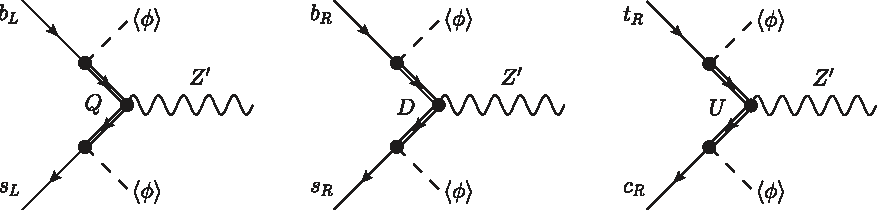
\includegraphics[width=\textwidth]{Bilder/NeueQuarks.pdf}
	\caption{Wechselwirkung von SM-Quarks mit dem Eichboson $Z'$ (aus \cite{InColour})}
\end{figure}
\end{frame}

\begin{frame}{Beschränkung der Parameter}
\framesubtitle{Zerfall $B\rightarrow K\bar{l}l$}
	\[ \SI{540}{\giga\electronvolt}\lessapprox\frac{m_{Z'}}{g'}\lessapprox\SI{4.9}{\tera\electronvolt} \]
\end{frame}

\begin{frame}{Beschränkung der Parameter}
\framesubtitle{Relic Density}
	\[ m_{Z'}\approx 2m_\chi \]
\end{frame}

\begin{frame}{Beschränkung der Parameter}
\framesubtitle{Direct Detection}
	\[ \SI{10}{\giga\electronvolt}\lessapprox m_{Z'} \lessapprox\SI{46}{\giga\electronvolt} \]
	\[ \SI{2e-3}{}\lessapprox g' \lessapprox\SI{e-2}{} \]
\end{frame}